\chapter{Analytical tools} \label{ch:Analytical tools}

A number of analytic tools will be utilized. The singular value decomposition and the numerical difficulties of direct inversion are covered in Section \ref{sec:SVD}; these numerical difficulties will motivate the need for regularization. Section \ref{sec:Tikhonov reg.} introduces Tikhonov regularization, as well as a discussion regarding the forms in which Tikhonov regularization can be stated.  To conclude the chapter, Section \ref{sec:Classes of matrices} presents some of the properties of a number of classes of matrices that will be used in later chapters.

\section{The Singular Value Decomposition} \label{sec:SVD}

Direct matrix inversion is not always practical, and not even possible when $\kMat$ can be singular. Fortunately, the singular value decomposition (SVD) of $\kMat$ can used instead if the system is not too large. Even for problems resulting in large discrete systems, the SVD is useful for analyzing solution methods.  Assuming $\kMat$ is a real $m \times n$ matrix, the SVD of $\kMat$ is
\begin{equation}
\kMat = U\Sigma{V^\trans}
\label{eq:SVD}
\end{equation}
where the $m \times m$ matrix $U$ and the $n \times n$ matrix $V$ have orthogonal columns and $\Sigma$ is a $m \times n$ diagonal matrix. The diagonal elements of $\Sigma$ are the singular values of $\kMat$, denoted $\singular_\ell$ and satisfying $\singular_0 \geq \singular_1 \geq \ldots \geq \singular_{n-1} \geq 0$. The columns of $U$ and $V$ will be denoted $U_{\cdot,\ell}$ and $V_{\cdot,\ell}$, respectively; these vectors are known as the left and right singular vectors of $\kMat$, respectively. A matrix of complex values has a SVD as well, the only difference being that the transpose is replaced with conjugate transpose. \par
Let $r$ denote the rank of $\kMat$. Then $\singular_0 \geq \ldots \geq \singular_{r-1} > 0$, i.e. the number of nonzero singular values of $\kMat$ is equal to the rank of $\kMat$.  A common variation of the SVD is the compact SVD (or economy SVD \cite{GolubVanLoan2013}), in which $\Sigma = \diag(\singular_0,\ldots,\singular_{r-1})$, $U$ is an $m \times r$ matrix and $V^\trans$ is an $r \times n$ matrix. The matrices $U$ and $V$ are no longer orthogonal in the traditional sense because they are not square (unless $\kMat$ is nonsingular). Instead, $U$ and $V$ are column orthonormal. \par 
By using $\kMat^{-1} = V\Sigma^{-1}U^\trans$ when $\kMat$ is nonsingular, the product $\kMat^{-1}\gnoiseVec$ is
\begin{equation}
\kMat^{-1}\gnoiseVec = \kMat^{-1}\left(\kMat\fVec + \noiseVec\right) = \fVec + \kMat^{-1}\noiseVec = \fVec + V\Sigma^{-1}{U^\trans}\noiseVec = \fVec + \sum_{\ell = 0}^{n-1} \frac{{U^\trans_\ell}\noiseVec}{\singular_\ell}V_{\cdot,\ell}. 
\label{eq:InvProd}
\end{equation}
Even if $\kMat$ is singular, a solution can still be obtained by using the pseudoinverse $\kMat^\dagger = V{\Sigma^\dagger}U^\trans$, where $\Sigma^\dagger = \diag(1/\singular_0,\ldots,1/\singular_{r-1})$, and the upper bound of summation in \eqref{eq:InvProd} becomes $r-1$. In either the nonsingular or singular case for $\kMat$, however, the summands in \eqref{eq:InvProd} are numerically unstable for small $\singular_\ell$. For a visual representation of this instability, a Picard plot can be constructed. A Picard plot is a graph showing the terms $|U^\trans_{\cdot,\ell}\noiseVec|/\singular_\ell$ in decreasing order with respect to the singular values. If the terms $|U^\trans_{\cdot,\ell}\noiseVec|$ decay faster than $\singular_\ell$ as $\ell$ increases, then the terms $|U^\trans_{\cdot,\ell}\noiseVec|/\singular_\ell$ do not become excessively large; this is the discrete Picard condition \cite{ABT}. The discrete Picard condition is thus a measure of instability. If the discrete Picard condition is not met, then the terms $|U^\trans_{\cdot,\ell}\noiseVec|/\singular_\ell$ blow up as $\ell$ increases, often resulting in worthless solutions. In this report, the discrete Fourier and cosine transforms will be used to obtain solutions analogous to those obtained by \eqref{eq:InvProd}. Figure \ref{PicardPlot} in Chapter \ref{ch:DFT} is an example of a Picard plot is provided that demonstrates the relationship between the noise, the width of the Gaussian blur, and the resulting numerical instabilities related to obtaining meaningful solutions. See \cite{Hansen1990} for more information on Picard plots and the associated discrete Picard condition. \par 
A common approach to overcome numerical instabilities is to multiply the summands in \eqref{eq:InvProd} by \textit{filter functions} $\filt$ that depend upon $\singular_\ell$ and a non-negative \textit{regularization parameter} $\regparam$. By doing so, an approximate solution is obtained:
\begin{equation}
\fVec_\regparam = \sum_{\ell = 0}^{n-1} V_{\cdot,\ell}\filt(\regparam,\singular_\ell)\left(\frac{{U^\trans_\ell}\gnoiseVec}{\singular_\ell}\right) = V\Phi\Sigma^\dagger U^\trans\gnoiseVec,
\label{eq:ApproxSol}
\end{equation}
where the matrix $\Phi$ is diagonal with $\Phi_{\ell,\ell} = \filt(\regparam,\singular_\ell)$ for $\ell = 0,\ldots,{n-1}$. The most desired property of the filter functions is that $\filt(\singular_\ell)/\singular_\ell \approx 1$  for large values of $\singular_\ell$ and $\filt(\singular_\ell)/\singular_\ell \approx 0$ for small values of $\singular_\ell$.  Perhaps the simplest filter function is
\[\filt(\regparam,\singular_\ell) = \begin{cases}
1, & \singular_\ell^2 > \regparam \\
0, & \singular_\ell^2 \leq \regparam
\end{cases}\]
Using this function in (3) gives the approximate solution
\[\fVec_\regparam = \sum_{\singular_\ell^2 > \regparam} \frac{{U^\trans_\ell}\gnoiseVec}{\singular_\ell}V_{\cdot,\ell}\]
which actually corresponds to the solution obtained using a truncated singular value decomposition (TSVD) of the matrix $\kMat$ \cite[p.~3-5]{Vogel:2002}. \par

\section{Tikhonov regularization} \label{sec:Tikhonov reg.}

A less simple filter function is
\begin{equation}
\filt(\regparam,\singular_\ell)  = \frac{\singular_\ell^2}{\singular_\ell^2 + \regparam^2}
\label{eq:TikFilt}
\end{equation}
which is known as the Tikhonov filter function. For large values of $\regparam$, \eqref{eq:TikFilt} is close to zero and for small values of $\regparam$ (and nonzero values of $\singular_\ell$), it is close to one. Another property of \eqref{eq:TikFilt} is that for fixed nonzero $\singular_\ell$, it is monotone decreasing in $\regparam$. Since the expression $1 - \filt(\regparam,\singular_\ell)$ arises a number of times in the methods introduced in Chapter \ref{ch:Parameter estimation methods}, let
\begin{equation}
\mfilt(\regparam,\singular_\ell) = 1 - \filt(\regparam,\singular_\ell) = \frac{\regparam^2}{\singular_\ell^2 + \regparam^2}.
\label{eq:TikFiltPsi}
\end{equation}
to simplify notation. In contrast to \eqref{eq:TikFilt}, \eqref{eq:TikFiltPsi} is close to one for large values of $\regparam$ and monotone increasing in $\regparam$ for fixed $\singular_\ell$; see Figure \ref{fig:Phi Psi Plot}. \par 

\begin{figure}
	\centerline{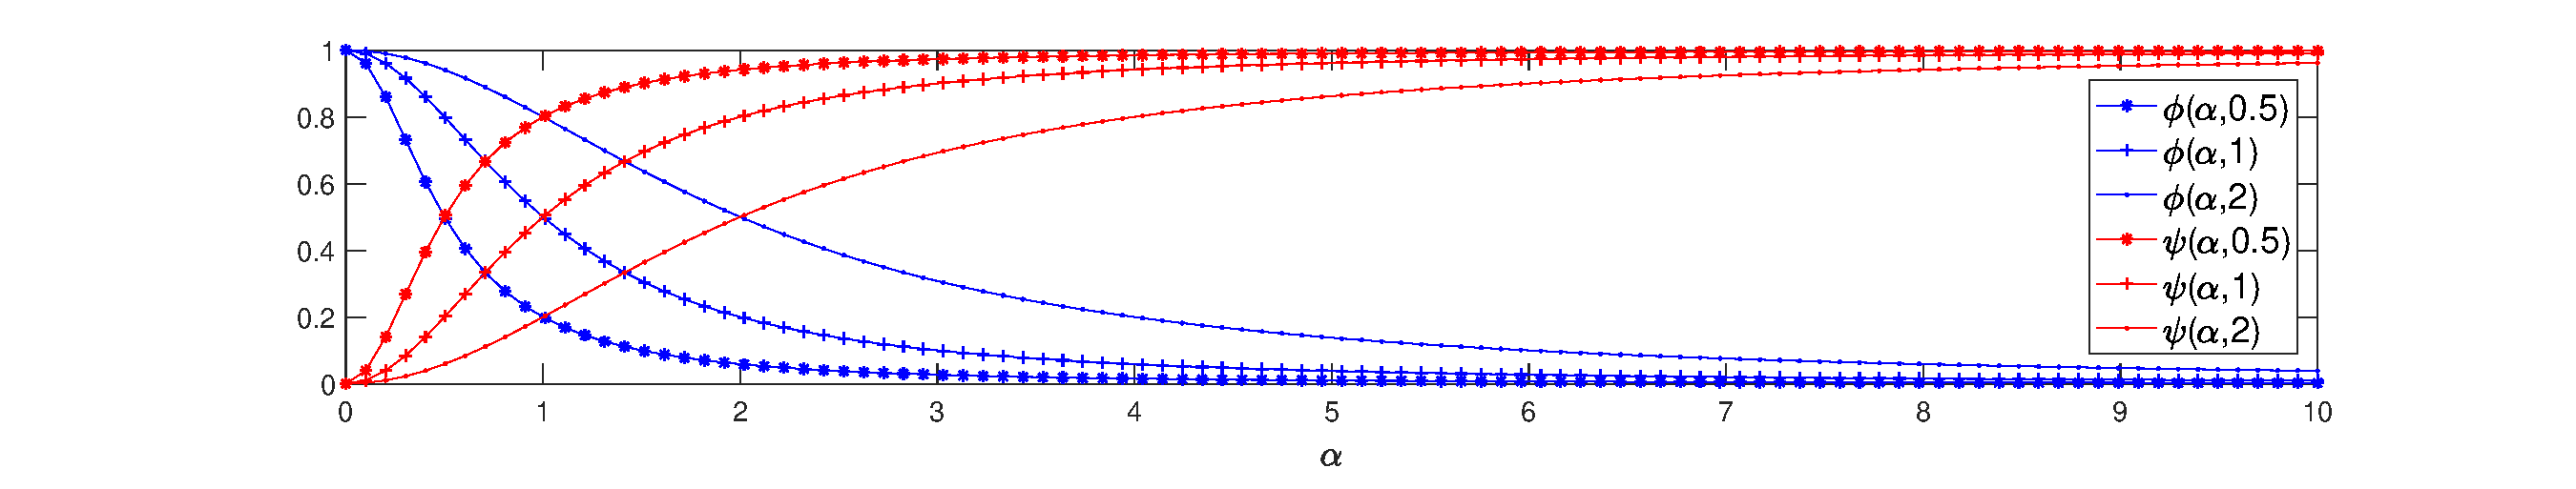
\includegraphics[scale = 0.4]{Figures/Phi_Psi_Plot.eps}}
\caption{The behavior of the Tikhonov filter function $\filt(\regparam,\singular_\ell)$ and corresponding $\mfilt(\regparam,\singular_\ell) = 1 - \filt(\regparam,\singular_\ell)$ is displayed for choice values of $\singular_\ell$. For fixed $\singular_\ell$, $\filt(\regparam,\singular_\ell) \rightarrow 0$ and $\mfilt(\regparam,\singular_\ell) \rightarrow 1$ as $\regparam \rightarrow \infty$. Notice also that $\filt(\regparam,\singular_\ell) = \mfilt(\regparam,\singular_\ell) = 1/2$ for $\alpha = \singular_\ell$.}
\label{fig:Phi Psi Plot}
\end{figure}

The use of the Tikhonov filter function to generate an approximate solution is known as \textit{Tikhonov regularization} \cite{Tikh1963}; in terms of an SVD, the obtained solution is
\begin{equation}
\fVec_\regparam = \sum_{\ell = 1}^n \filt(\regparam,\singular_\ell)\frac{{U^\trans_\ell}\gnoiseVec}{\singular_\ell}V_{\cdot,\ell} = \sum_{\ell = 0}^{n-1} \frac{\singular_\ell{U^\trans_\ell}\gnoiseVec}{\singular_\ell^2 + \regparam^2}V_{\cdot,\ell} = V\Phi\Sigma^\dagger U^\trans\gnoiseVec.
\label{eq:TikSol}
\end{equation}
An alternative (and more general) representation of the above Tikhonov solution is
\begin{equation}
\fVec_\regparam = \argmin_{\fVec \in \mathbb{R}^n} \left\{\|\kMat\fVec - \gnoiseVec\|^2 + \regparam^2\|D\fVec\|^2\right\},
\label{eq:TikSol2}
\end{equation}
where $D$ is the matrix representation of a linear operator and $\|\cdot\|$ is the 2-norm. The term $\|D\fVec\|^2$ is commonly called the penalty function \cite{Vogel:2002}. The representation \eqref{eq:TikSol} follows from selecting $D$ to be $I$, the $n \times n$ identity matrix. The solution \eqref{eq:TikSol2} can also be expressed in block form as
\begin{equation}
\fVec_\regparam = \argmin_{\fVec \in \mathbb{R}^n} \left\| \begin{bmatrix}
\kMat \\
\regparam D
\end{bmatrix}\fVec - \begin{bmatrix}
\gnoiseVec \\
\zeroVec
\end{bmatrix} \right\|^2.
\label{eq:TikSol3}
\end{equation}
If the matrix $D$ in \eqref{eq:TikSol2} is non-singular, then the substitutions $\mathbf{y} = D\fVec$, $A = \kMat{D}^{-1}$, and $\mathbf{b} = \gnoiseVec$ give
\begin{equation}
\mathbf{y}(\regparam) = \argmin_{\mathbf{y} \in \mathbb{R}^n} \|A\mathbf{y} - \mathbf{b}\|^2 + \regparam^2\|\mathbf{y}\|^2.
\label{eq:TikSol Standard Form}
\end{equation}
This is known as standard form of the regularization problem. Once $\mathbf{y}$ is obtained from \eqref{eq:TikSol Standard Form}, the final solution is recovered by $\fVec = D^{-1}\mathbf{y}$.  \par 
However, there are many examples of matrices $D$ that are singular, such as finite difference matrices that approximate derivative operators. In such cases, the regularization can still be recast in standard form, which can be accomplished in a convenient way using the generalized singular value decomposition (GSVD). To simplify the derivation of the GSVD, it will be assumed that the matrix $[\kMat, \regparam D]^\trans$ in \eqref{eq:TikSol3} has full column rank, i.e. $\nullspace(\kMat) \cap \nullspace(D) = \varnothing$, which ensures that the solution $\fVec_\regparam$ is unique. Another simplifying assumption being that the $p \times n$ matrix $D$ with $p \leq n$ has full row rank. Under these assumptions \cite[p.~104]{ABT}, the matrices $\kMat$ and $D$ can be expressed as
\begin{equation}
\label{eq:GSVD matrices}
\kMat = U\Lambda X^\trans, \quad D = VMX^\trans
\end{equation}
where the matrices $U$, $V$, $\Lambda$, $M$, and $X$ satisfy the following: 
\begin{itemize}
\item $U$ is an orthogonal $m \times m$ matrix. 
\item $V$ is an orthogonal $p \times p$ matrix.
\item $\Lambda$ is an $m \times n$ matrix with the property that the nonzero entries satisfy
\[0 \leq \Lambda_{1,k+1} \leq \ldots \leq \Lambda_{m,k+m} \leq 1,\]
where $k = 0$ if $m > n$ and $k = n-m$ otherwise. 
\item $M$ is a diagonal $p \times n$ matrix with $M_{1,1} \geq \ldots \geq M_{p,p} \geq 0.$
\item $M^\trans M + \Lambda^\trans \Lambda = I$ (the dimension of the identity matrix being $n \times n$).
\item $X$ is a nonsingular $n \times n$ matrix.
\end{itemize}
The generalized singular values of $\kMat$ and $D$ are defined as $\gamma_\ell = \lambda_{\ell}/\mu_{\ell}$, where
\begin{equation}
\label{eq:GSVD lambda}
\lambda_\ell = \sqrt{(\Lambda^\trans \Lambda)_{\ell,\ell}}, \quad \mu_\ell = \sqrt{(M^\trans M)_{\ell,\ell}}
\end{equation}
for $\ell = 0,\ldots,{n-1}$. In contrast to the SVD, the generalized singular values are ordered $\gamma_0 \leq \ldots \leq \gamma_{n-1}$. It is also possible that $\mu_\ell = 0$ for some $\ell$, in which case $\gamma_\ell$ is not defined. Even when $\mu_\ell$ is small the resulting value of $\gamma_\ell$ can be excessively large, again emphasizing the need for regularization. By applying the orthogonality properties of the GSVD matrices \cite[p.~105-106]{ABT}, the regularized solution \eqref{eq:TikSol3} can be expressed as
\begin{equation}
\label{eq:TikSol GSVD}
\fVec_\regparam = \sum_{\ell=0}^{n-1} \frac{\gamma_\ell^2}{\gamma_\ell^2 + \regparam^2} \frac{U_{\cdot,\ell+k}^\trans\gnoiseVec}{\lambda_\ell}Y_{\cdot,\ell}
\end{equation}
where $Y = X^{-\trans}$ (the inverse of $X^\trans$). The terms $\gamma_\ell^2/(\gamma_\ell^2 + \regparam^2)$ are known as the GSVD filter factors, which are identical in form to the filter factors \eqref{eq:TikFilt}. \par 
With the derivation of the GSVD established, an extension of the transformation that rendered \eqref{eq:TikSol Standard Form} is now stated \cite[p.~38]{Hansen:98}. First, a weighted version of the pseudoinverse $D^\dagger$ is defined as
\[D_{\kMat}^\dagger = \left(I - \left(\kMat\left(I - D^\dagger D\right)\right)^\dagger \kMat\right)D^\dagger.\]
If $p \geq n$, then $D_{\kMat}^\dagger$ is the same as $D^\dagger$. We must also consider
\[\fVec_0 \equiv \left(\kMat\left(I - D^\dagger D\right)\right)^\dagger \gnoiseVec,\]
which is the component of the solution contained in $\nullspace(D)$.  Using the GSVD matrices from \eqref{eq:GSVD matrices}, $D_{\kMat}^\dagger$ and $\fVec_0$ can be written as
\begin{equation}
\label{eq:Trans. 1}
D_{\kMat}^\dagger = X \begin{bmatrix}
M^{-1} \\
\mathbf{0}
\end{bmatrix}V^\trans, \quad \fVec_0 = \sum_{\ell=m+1}^{n} U_{\cdot,\ell}^\trans\gnoiseVec X_{\cdot,\ell}
\end{equation}
where $\zeroVec$ is the zero matrix of appropriate dimension. The form of the regularized solution can be expressed as \eqref{eq:TikSol Standard Form} with substitutions $\mathbf{y} = D\fVec$, $A = \kMat{D_{\kMat}^\dagger}$, and $\mathbf{b} = \gnoiseVec - \kMat\fVec_0$. 
%This is shown by writing
%\begin{align*}
%\|A\mathbf{y} - \mathbf{b}\|^2 + \regparam^2\|\mathbf{y}\|^2 &= \|\kMat{D_{\kMat}^\dagger}D\fVec - (\gnoiseVec - \kMat\fVec_0)\|^2 + \regparam^2\|D\fVec\|^2 \\
%&=  \|\kMat({D_{\kMat}^\dagger}D\fVec + \fVec_0) - \gnoiseVec\|^2 + \regparam^2\|D\fVec\|^2
%\end{align*}
%as well as 
%\ToDo{
%\begin{align*}
%{D_{\kMat}^\dagger}D\fVec + \fVec_0 &= \left(I - \left(\kMat\left(I - D^\dagger D\right)\right)^\dagger \kMat\right)D^\dagger D\fVec + \left(\kMat\left(I - D^\dagger D\right)\right)^\dagger \gnoiseVec \\
%&= D^\dagger D\fVec - \left(\kMat\left(I - D^\dagger D\right)\right)^\dagger \kMat D^\dagger D\fVec + \left(\kMat\left(I - D^\dagger D\right)\right)^\dagger \gnoiseVec \\ 
%&= D^\dagger D\fVec + \left(\kMat\left(I - D^\dagger D\right)\right)^\dagger \left[\gnoiseVec - \kMat D^\dagger D\fVec\right] \\
%&= 
%\end{align*}}
The final solution is then recovered by $\fVec = D_{\kMat}^\dagger \mathbf{y} + \fVec_0$. 

%\section{Discrete convolution} \label{sec:Discrete convolution}
%As described in the Chapter \ref{ch:Introduction}, the operation of convolution arises in various settings pertaining to inverse problems. Discrete convolution will first be described  in a general setting, followed by specific instances and connections to appropriate numerical examples. \par
%Let $(x_n)$ and $(y_n)$ be sequences of complex numbers indexed by the integers. Then the discrete convolution of $(x_n)$ and $(y_n)$, denoted $x*y$, is defined by
%\[(x*y)_n = \sum_{\ell=-\infty}^\infty x_{n-\ell}y_\ell.\]
%The series in the definition of discrete convolution is bi-infinite, meaning that the discrete convolution might not be well-defined for any two arbitrary sequences. For example, if $x_n = y_n = 1$ for all $n \in \mathbb{Z}$, then the series defining $(x*y)_n$ is $\sum_{j=-\infty}^\infty 1$, which does not converge. In various cases, however, the discrete convolution is well-defined. These cases include sequences having only finitely-many nonzero terms and sequences in $\ell^1$. (In fact, the set of sequences having finitely-many nonzero terms is a linear subspace of $\ell^1$).  \par 
%Fortunately, real-world applications usually involve finite sequences (vectors), which can be thought of as infinite or bi-infinite sequences having finitely-many nonzero terms. While such sequences do not require the evaluation of infinite series to compute discrete convolutions, it is helpful to have general results regarding the length and indices of discrete convolutions. Let $(x_n)$ and $(y_n)$ be nonzero sequences with finitely-many nonzero terms. For $(x_n)$, the assumptions imply the existence of integers $b_x$ and $e_x$ such that $x_n = 0$ for all $n \in \mathbb{Z}$ with either $n < b_x$ or $e_x < n$. Such integers exist for $(y_n)$ and will be denoted $b_y$ and $e_y$. The choice of letters reflects the fact that $s$ and $e$ represent the starting and ending indices of the section of the sequence where the terms can be nonzero. Extending this notation, the number of terms in this section of sequence is $n_x = e_x - b_x + 1$ and $n_y = e_y - b_y + 1$ for $(x_n)$ and $(y_n)$, respectively. From \cite{BoggessNarcowich2009}, the values of $s_{x*y}$, $e_{x*y}$, and $n_{x*y}$ are
%\begin{align}
%s_{x*y} &= b_x + b_y, \nonumber \\
%e_{x*y} &= e_x + e_y, \label{eq:FIEResults} \\
%n_{x*y} &= n_x + n_y - 1. \nonumber
%\end{align}
%As an illustrative example, let $\mathbf{x} = [1,2,3]$ and $\mathbf{y} = [4,5,6,7]$ be row vectors. The vectors can be thought of as the bi-infinite sequences $(x_n) = (\ldots,0,1,2,3,0\ldots)$ and $(y_n) = (\ldots,0,4,5,6,7,0,\ldots)$. If the sequences are indexed so that $x_1 = 1$ and $y_1 = 4$, then $b_x = b_y = 1$, $e_x = n_x = 3$, and $e_y = n_y = 4$. Then by \eqref{eq:FIEResults}, $s_{x*y} = 2$, $e_{x*y} = 8$, and $n_{x*y} = 6$. The bi-infinite sequence produced from the convolution is
%\[x*y = (\ldots,0,4,13,28,34,32,21,0,\ldots),\]
%where $(x*y)_2 = 4$ and $(x*y)_8 = 21$. \par 
%Since the numerical examples are conducted in MATLAB, a brief remark regarding discrete convolutions in MATLAB is be given. If the built-in function \texttt{conv} is used to evaluate the discrete convolution of row vectors $\mathbf{x}$ and $\mathbf{y}$ described in the previous example, the output is the row vector $[4,13,28,34,32,21]$.  All vectors in MATLAB have a starting index of 1, and the vector resulting from the convolution is no different: the component 4 has an index of 1. While this seems to conflict with \eqref{eq:FIEResults} (recall that $s_{x*y} = 2$, not 1), from a practical standpoint there is little reason for concern; usually the components themselves are of interest and not the indexing of the bi-infinite sequence. If one wants to keep track of the indexing as the convolution is evaluated, index vectors can be defined for $\mathbf{x}$ and $\mathbf{y}$ and \eqref{eq:FIEResults} can be applied to obtain an index vector for the resulting convolution. See \cite{BoggessNarcowich2009} for an explicit MATLAB example. \par 

\section{Classes of matrices} \label{sec:Classes of matrices}
The first type of matrix to be discussed is a \textit{Toeplitz matrix}. A matrix $T$ is called a Toeplitz matrix if it is constant along each diagonal. The following are examples of Toeplitz matrices:
\[A = \begin{bmatrix}
1 & 2 \\
3 & 1 \\
0 & 3
\end{bmatrix}, \quad 
B = \begin{bmatrix}
4 & 8 & 5 \\
7 & 4 & 8 \\
1 & 7 & 4
\end{bmatrix}.\]
By definition, Toeplitz matrices need not be square. However if a Toeplitz matrix is square with dimension $n \times n$, then it is uniquely determined by $2n-1$ entries. If a Toeplitz matrix is symmetric, then it is determined by $n$ entries. \par
Some notation for symmetric Toeplitz matrices will be introduced that will be used in Chapter \ref{ch:DCT}. Given a column vector $\mathbf{v}$ of length $n$, let $T(\mathbf{v})$ denote the $n \times n$ symmetric Toeplitz matrix with $\mathbf{v}$ as its first column. As example, the matrix $T(\mathbf{v})$ where $\mathbf{v} = [1,2,3,4]^\trans$ is
\[T(\mathbf{v}) = \begin{bmatrix}
1 & 2 & 3 & 4 \\
2 & 1 & 2 & 3 \\
3 & 2 & 1 & 2 \\
4 & 3 & 2 & 1 
\end{bmatrix}.\] 
The primary connection to be made is that discrete convolutions can be described in the context of matrix-vector multiplication using Toeplitz matrices. For example, the discrete convolution of $\mathbf{x} = [1,2,3]$ and $\mathbf{y} = [4,5,6]$ can be cast as a matrix-vector product by defining a matrix $X$ to be
\[X = \begin{bmatrix}
1 & 0 & 0  \\
2 & 1 & 0 \\
3 & 2 & 1 \\
0 & 3 & 2 \\
0 & 0 & 3 
\end{bmatrix}.\]
Certainly $X$ is a Toeplitz matrix, and $x*y$ can be expressed as $Xy^\trans$ with $x*y$ being a (column) vector of length $n_{x*y} = 6$. The operation $Xy^\trans$ is equivalent to \texttt{conv(x,y)} in MATLAB. \par 
A type of matrix that is closely related to Toeplitz matrices is a Hankel matrix. A Hankel matrix is a matrix that is constant along each anti-diagonal. The following are examples of Hankel matrices:
\[A = \begin{bmatrix}
-1 & 2 \\
2 & 0 \\
0 & -6
\end{bmatrix}, \quad 
B = \begin{bmatrix}
1 & 2 & 5 \\
2 & 5 & 3 \\
5 & 3 & 9
\end{bmatrix}.\]
Similar to square Toeplitz matrices, a square Hankel matrix with dimension $n \times n$ is uniquely defined by $2n -1$ entries and symmetric Hankel matrices are determined by $n$ entries. Extending the notation for symmetric Toeplitz matrices, let $H(\mathbf{v})$ be the $n \times n$ symmetric Hankel matrix with the $n$-vector $\mathbf{v}$ as its first column. \par
A specific type of square Hankel matrix is the exchange matrix $J$, defined by ones along the main anti-diagonal and zero elsewhere. As a visual, the $4 \times 4$ exchange matrix is
\[J = \begin{bmatrix}
0 & 0 & 0 & 1 \\
0 & 0 & 1 & 0 \\
0 & 1 & 0 & 0 \\
1 & 0  & 0 & 0
\end{bmatrix}.\]
The exchange matrix is so-named for the property that the product of $J$ with a vector $\mathbf{v}$ has the effect of ``exchanging" (or ``reversing") the entries of $\mathbf{v}$. For example, if $\mathbf{v} = [1,2,3,4]^\trans$ then $J\mathbf{v} = [4,3,2,1]^\trans$. As a result of this property, the exchange matrix is an involution, i.e. $J^2 = I$. Another result of the properties of $J$ is that the product of a Toeplitz matrix with the exchange matrix is a Hankel matrix. Lemma \ref{lem:TJ = H} outlines a specific case where the Toeplitz matrix is symmetric.
\begin{lemma}
\label{lem:TJ = H}
Let $\mathbf{v} \in \mathbb{R}^n$ and let $J$ be the $n \times n$ exchange matrix. Then $T(J\mathbf{v})J = H(\mathbf{v})$.
\end{lemma}
\begin{proof}
By the symmetry of $T(J\mathbf{v})J$, it suffices to argue that the first column of $T(J\mathbf{v})J$ is $\mathbf{v}$. Since $T(J\mathbf{v})$ is post-multiplied by $J$, the first column of the product is equal to the last column of $T(J\mathbf{v})$. By definition, the last column of $T(J\mathbf{v})$ is $J(J\mathbf{v}) = J^2\mathbf{v} = \mathbf{v}$.
\end{proof}
If a matrix $C$ has the property that each row is the circular right shift of the components of the preceding row, then $C$ is called a \textit{circulant matrix}. The \textit{circular right shift} of a row vector $[x_0,x_1,\ldots,x_{n-1}]$ is $[x_{n-1},x_0,\ldots,x_{n-2}]$. From this definition, every circulant matrix is also a Toeplitz matrix. For example,
\[C = \begin{bmatrix}
1 & 2 & 3 & 4 \\
4 & 1 & 2 & 3 \\
3 & 4 & 1 & 2 \\
\end{bmatrix}\] 
is a circulant matrix generated by circular right shifts of the vector $[1,2,3,4]$. A final observation regarding circulant matrices can be made about their indexing. If $\mathbf{c} = [c_0,\cdots,c_{n-1}]$ is the first row of a circulant matrix $C$, then
\begin{equation}
\label{eq:Circulant indexing}
C_{j,k} = c_{k-j \bmod n}
\end{equation}
for all $0 \leq j,k \leq n-1$. A significant property of square circulant matrices discussed in Chapter \ref{ch:DFT} is that they are diagonalized by the discrete Fourier transform; \eqref{eq:Circulant indexing} can be used to prove this property.

\section{Discrete trigonometric transforms} \label{sec:Discrete trig. transforms}

The discrete Fourier transform will be introduced from the perspective of approximating coefficients of the Fourier series of a $2\pi$-periodic function $f$ \cite[p.~132-134]{BoggessNarcowich2009}. On the interval $[0,2\pi]$, the $j$th complex Fourier coefficient of $f(t)$ is given by
\[c_j = \frac{1}{2\pi}\int_0^{2\pi} f(t)\exp(-ijt)\:dt,\]
where $i = \sqrt{-1}$.  Applying the trapezoidal rule for approximating this integral with $n$ points then produces
\[c_j \approx \frac{1}{n}\sum_{\ell = 0}^{n-1} f\left(\frac{2\pi{\ell}}{n}\right)\exp\left(\frac{-2\pi{ij\ell}}{n}\right).\]
The \textit{discrete Fourier transform} (DFT) is a mapping $\mathcal{F}:\mathbb{C}^n \rightarrow \mathbb{C}^n$ defined by
\begin{equation}
\mathcal{F}(\mathbf{f})_j = \frac{1}{\sqrt{n}}\sum_{\ell=0}^{n-1} f_{\ell}\exp\left(\frac{-2\pi{ij\ell}}{n}\right), \quad \mathbf{f}\in\mathbb{C}^n, \quad 0 \leq k \leq n-1.
\label{eq:DFT}
\end{equation}
The DFT of a vector $\mathbf{f}$ will be denoted by $\dft{\mathbf{f}}$. The inverse DFT of a vector $\dft{\mathbf{f}}$ is given by
\begin{equation}
\mathcal{F}^{-1}(\dft{\mathbf{f}})_j = \frac{1}{\sqrt{n}}\sum_{\ell=0}^{n-1} \dft{f}_\ell\exp\left(\frac{2\pi{ij\ell}}{n}\right) = f_j.
\end{equation}
These definitions are nonstandard; typically the factors $1/\sqrt{n}$ in both the forward and inverse DFT definitions are combined as a single factor of $1/n$ in the definition of the forward DFT. The DFT can also be stated in terms of matrix-vector multiplication. Given an $\mathbf{f} \in \mathbb{C}^n$, $\dft{\mathbf{f}}$ can be expressed as $F\mathbf{f}$ where the matrix $F\in\mathbb{C}^{n\times{n}}$ has components
\begin{equation}
F_{j,k} = \frac{1}{\sqrt{n}}\exp\left(\frac{-2\pi{ijk}}{n}\right), \quad 0 \leq j,k \leq n-1.
\label{eq:DFT-Matrix}
\end{equation}
The matrix representing the inverse DFT is then $F^\ctrans$, where $\ctrans$ denotes conjugate transposition. A property of $F$ is that $F^\ctrans F = FF^\ctrans = (1/n)\diag(n) = I$, and so splitting the factor of $1/n$ as $(1/\sqrt{n})(1/\sqrt{n})$ for the definition of the DFT provides the benefit of $F$ being a unitary matrix. A direct consequence of the DFT being unitary is Parseval's theorem: $\|\mathbf{f}\| = \|F\mathbf{f}\|$ for any $\mathbf{f} \in \mathbb{C}^n$. Parseval's theorem follows directly from \eqref{eq:DFT} because
\begin{align*}
\|F\mathbf{f}\|^2 &= \sum_{\ell=0}^{n-1} |\mathcal{F}(\mathbf{f})_\ell |^2 \\
&= \sum_{\ell=0}^{n-1} \left(\frac{1}{\sqrt{n}}\sum_{j=0}^{n-1} f_{j}\exp\left(\frac{-2\pi{ij\ell}}{n}\right)\right)\overline{\left(\frac{1}{\sqrt{n}}\sum_{j'=0}^{n-1} f_{j'}\exp\left(\frac{-2\pi{ij'\ell}}{n}\right)\right)} \\
&= \frac{1}{n} \sum_{\ell=0}^{n-1} \left(\sum_{j=0}^{n-1} f_{j}\exp\left(\frac{-2\pi{ij\ell}}{n}\right)\right) \left(\sum_{j'=0}^{n-1} \overline{f_{j'}}\exp\left(\frac{2\pi{ij'\ell}}{n}\right)\right) \\
&= \frac{1}{n} \sum_{\ell=0}^{n-1} \left(\sum_{j=0}^{n-1} f_{j} \sum_{j'=0}^{n-1} \overline{f_{j'}} \exp\left(\frac{2\pi{i(j'-j)\ell}}{n}\right)\right) \\
&= \frac{1}{n} \sum_{j=0}^{n-1} f_j \sum_{j'=0}^{n-1} \overline{f_{j'}} \sum_{\ell=0}^{n-1} \exp\left(\frac{2\pi{i(j'-j)\ell}}{n}\right).
\end{align*}
Since the innermost sum is geometric,
\[\sum_{\ell=0}^{n-1} \exp\left(\frac{2\pi{i(j'-j)\ell}}{n}\right) = \begin{cases}
\frac{\exp(2\pi{i}(j-j')) - 1}{\exp(2\pi{i}(j-j')/n) - 1} = 0, & j \neq j' \\
n, & j = j'
\end{cases}.\]
Therefore
\[\|F\mathbf{f}\|^2 = \frac{1}{n} \sum_{j=0}^{n-1} f_j \sum_{j'=0}^{n-1} \overline{f_{j'}} \sum_{\ell=0}^{n-1} \exp\left(\frac{2\pi{i(j'-j)\ell}}{n}\right) = \sum_{j=0}^{n-1} f_j\overline{f_j} = \|\mathbf{f}\|^2,\]
which proves Parseval's theorem. \par
As stated previously, a significant property of circulant matrices is that they are diagonalized by the DFT. Using the definition of the $n \times n$ unitary Fourier matrix $F$, the property can be stated as
\begin{equation}
C = F^\ctrans\diag(\sqrt{n}\dft{\mathbf{c}})F,
\label{eq:CircDiag}
\end{equation}
where $C$ is any $n \times n$ circulant matrix and $\dft{\mathbf{c}}$ is the DFT of the first row of $C$ (recall that the rows of a circulant matrix are circulant right shifts of a single row vector of length $n$). This property can be shown directly by showing that $C_{j,k} = (F^\ctrans\diag(\dft{\mathbf{c}})F)_{j,k}$ for any $0 \leq j,k \leq n-1$. Using the definition of the DFT and \eqref{eq:Circulant indexing}, the component of $F^\ctrans\diag(\sqrt{n}\dft{\mathbf{c}})F$ in $j$th row and $k$th column is given by
\begin{align*}
\sum_{\ell=0}^{n-1} \left[\frac{1}{\sqrt{n}}  \exp\left(\frac{2\pi{i}k\ell}{n}\right)\right] \left[\sqrt{n}\dft{c}_\ell\right] \left[\frac{1}{\sqrt{n}} \exp\left(\frac{-2\pi{i}j\ell}{n}\right)\right] &= \frac{1}{\sqrt{n}} \sum_{\ell=0}^{n-1} \dft{c}_\ell \exp\left(\frac{2\pi{i}(k-j)\ell}{n}\right) \\
&= c_{k-j \bmod n} \\
&= C_{j,k}.
\end{align*}
It should be noted that by defining the DFT with the factor of $1/n$ as part of the inverse transformation (while keeping the factor split as $(1/\sqrt{n})(1/\sqrt{n})$ in the matrix form) would allow the property to be stated simply as $C = F^\ctrans\diag(\dft{\mathbf{c}})F$. \par 
Now the properties of the DFT will be connected with the SVD of a circulant matrix, which will be the basis for the design of the numerical examples in \ref{sec:Numerical results (DFT)}. Let $\fVec$ and $\kVec$ be the $N$-point discretizations of functions $f$ and $k$ on some interval $[a,b]$. Then the cyclic convolution $\gVec = \kVec * \fVec$ can be computed as a matrix-vector product by constructing an $N \times N$ circulant matrix $\kMat$ from $\kVec$. This construction is carried out by setting the first row of $\kMat$ to be $\kVec$, and each subsequent row to be a circular right shift of the preceding row (see \ref{sec:Classes of matrices}). In MATLAB, the command \texttt{toeplitz([k(1) fliplr(k(2:end))], k)} constructs the matrix $\kMat$. Then $\gVec = \kMat\fVec$, and after the addition of noise the equation \eqref{eq:DisNoise} is obtained. Then by using the property \eqref{eq:CircDiag} with the $N \times N$ unitary Fourier matrix $F$ and assuming that $\kMat$ is invertible, 
\begin{equation}
\kMat^{-1}\gnoiseVec = \fVec + (F^\ctrans\diag(\dft{\kVec})F)^{-1}\noiseVec = \fVec + F^\ctrans\diag(\dft{\kVec})^{-1}F\noiseVec = \fVec + \sum_{\ell = 0}^{n-1} F^\ctrans_{\ell,\cdot}\left(\frac{\dft{\noise}_\ell}{\dft{k}_\ell}\right),
\label{eq:InvProdDFT}
\end{equation}
where $\dft{\noise}_\ell$ and $\dft{k}_\ell$ are the $\ell$th Fourier coefficients of $\noiseVec$ and $\kVec$, respectively, and $F^\ctrans_{\ell,\cdot}$ is the conjugate transpose of the $\ell$th row of $F$ (i.e. the $\ell$th column of the matrix $F^\ctrans$). Analogous to \eqref{eq:InvProd}, instabilities can arise if $\dft{k}_\ell$ is small. By introducing filter factors to reduce possible instability, an approximate solution
\begin{equation}
\fVec_\regparam = \sum_{\ell = 0}^{n-1} F^\ctrans_{\ell,\cdot}\left(\frac{\filt(\regparam,\dft{k}_\ell)\dft{\gnoise}_\ell}{\dft{k}_\ell}\right) = F^\ctrans\Phi\dft{\kMat}^\dagger F\gnoiseVec
\label{eq:ApproxSolDFT}
\end{equation}
can be obtained analogous to \eqref{eq:ApproxSol}, where $\dft{\kMat}^\dagger = \diag(1/\dft{\kVec})$.
Since $F^\ctrans$ is a matrix representation of the inverse DFT, the approximate solution can be rewritten as
\[\fVec_\regparam = F^\ctrans \frac{\filt(\regparam,\dft{\kVec})\dft{\gnoiseVec}}{\dft{\kVec}}.\]
Here $\filt(\regparam,\dft{\kVec})\dft{\gnoiseVec}/{\dft{\kVec}}$ is a vector where the operations of multiplication and division are performed component-wise. This representation is useful for making a connection with the MATLAB implementation. \par
As mentioned in Chapter \ref{ch:Introduction}, a Picard plot is often useful in analyzing the numerical instabilities of solutions obtained from either or \eqref{eq:InvProd} or \eqref{eq:InvProdDFT}. Figure \ref{PicardPlot} shows an example of a Picard plot. The terms $|\dft{k}_\ell|$ decrease down to machine precision, though the $|\dft{\gnoise}_\ell|$ decrease but then level off just above the variance in the noise. As a result, the terms $|\dft{\gnoise}_\ell|/|\dft{k}_\ell|$ only decrease so far and then begin increasing. The steady increase can produce a blow up of the approximate solution. While illustrating these relationships, a Picard plot is also useful in determining how to truncate the sum in \eqref{eq:ApproxSolDFT} to avoid blow up in the solution. For the plot in Figure \ref{PicardPlot}, the sum in \eqref{eq:ApproxSolDFT} should be truncated around index 8 to obtain a meaningful solution. \par 

\begin{figure}[htb]
	\centerline{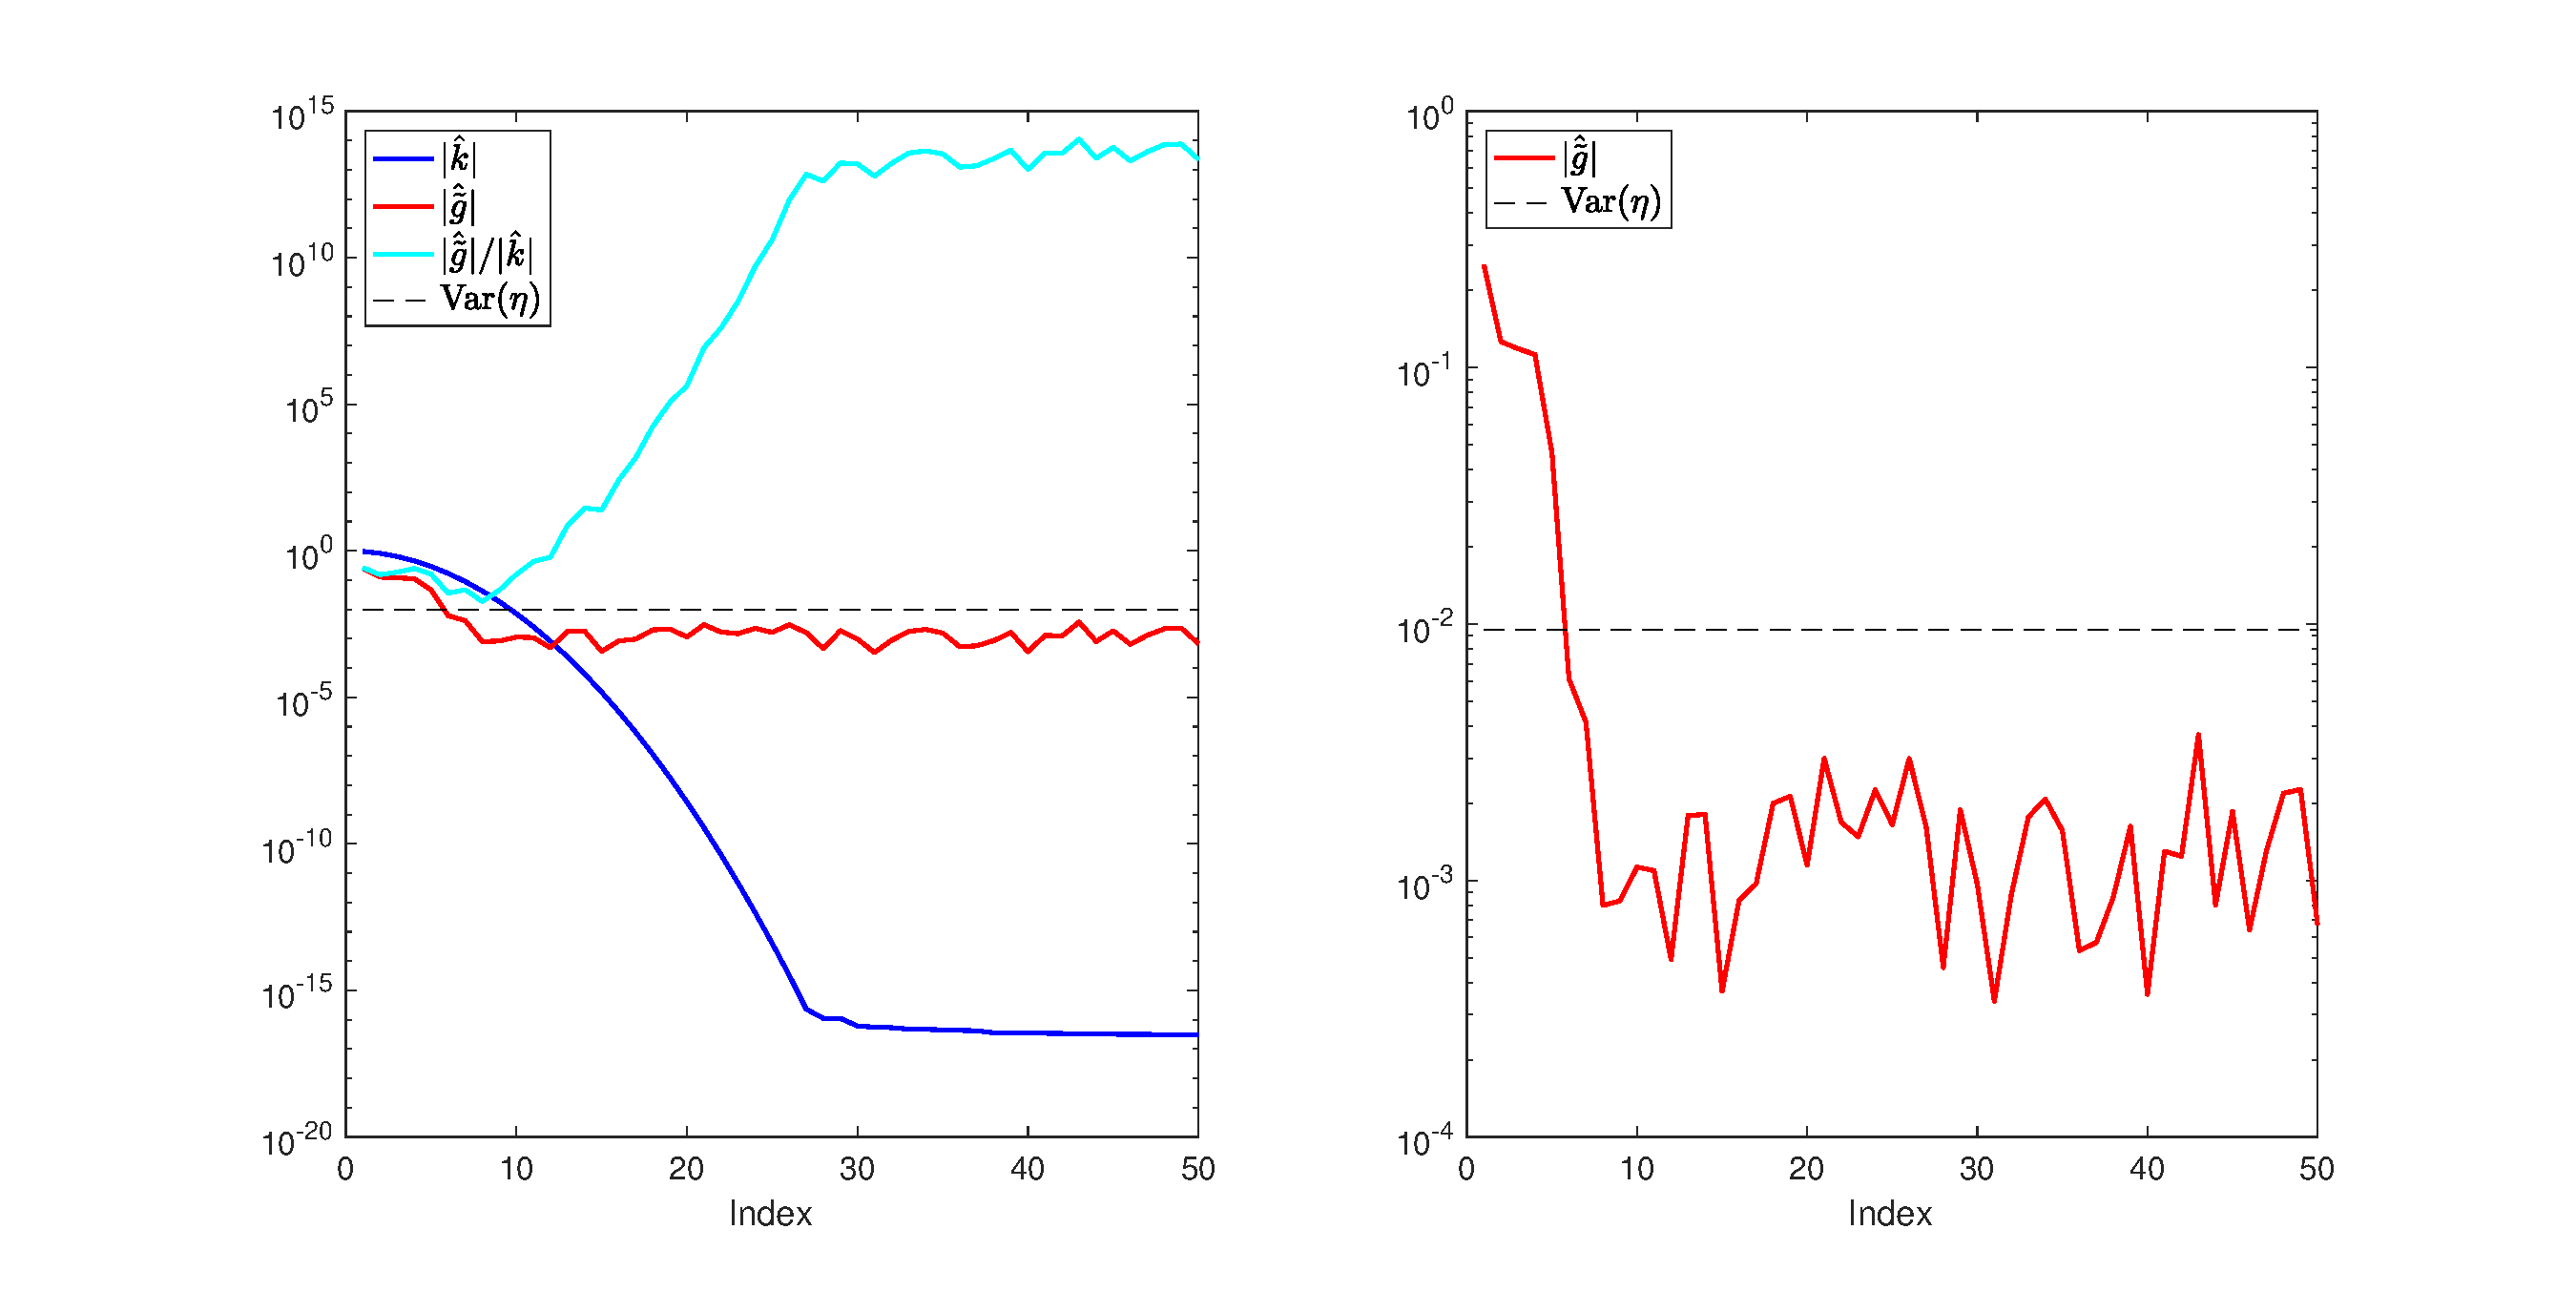
\includegraphics[scale = 0.45]{Figures/PicardPlot1D_F2_S15_W200.eps}}
\caption{(Left) A Picard plot generated from the second test function, a Gaussian blur with a width of 200, and an SNR of 15. The terms $|\dft{\gnoise}_\ell|/|\dft{k}_\ell|$ decrease until index 8, at which case the terms increase in magnitude. This is due to the fact that the $|\dft{k}_\ell|$ steadily decrease, while the $|\dft{\gnoise}_\ell|$ level off just below the variance in the noise. (Right) A zoom-in of the Picard plot is provided, showing that elements of the DFT of $\gnoiseVec$ decay only slightly below the variance of the noise in $\gnoiseVec$.}
\label{PicardPlot}
\end{figure}

While the connection between lines \eqref{eq:InvProdDFT} and \eqref{eq:ApproxSolDFT} and the SVD have been noted in regard to the structure of the terms and equations, a complete connection can be made if another property about $\kMat$ is assumed. Until this point $\kMat$ is assumed to be an invertible $N \times N$ circulant matrix formed from a vector $\kVec$. If $\kMat$ is also assumed to be symmetric, then the SVD of $\kMat$ is the same as the diagonalization by the unitary DFT matrix $F$ and the singular values of $\kMat$ are also the eigenvalues. \par 
Analogous to the DFT, the discrete cosine transform (DCT) can be introduced from the perspective of approximating the coefficients of a cosine series. Given a function $f(t)$ defined on the interval $[0,1]$, consider the even extension of $f_e(t)$ defined by
\[f_e(t) = \begin{cases}
f(t), & 0 \leq t \leq 1 \\
f(-t), & -1 \leq t < 0
\end{cases}.\]
From \cite[p.~49]{BoggessNarcowich2009}, the Fourier series expansion of $f_e(t)$ will only contain cosine terms and the coefficients of these terms are
\begin{align*}
a_0 &= \int_0^1 f(t)~dt, \\
a_j &= 2\int_0^1 f(t) \cos(j\pi{t})~dt, \quad j \leq 1.
\end{align*}
Approximating the integral for $a_j$ with $j \geq 1$ using the midpoint rule with $N$ subintervals of $[0,1]$ gives
\[a_j \approx \frac{2}{N}\sum_{k=0}^{N-1} f\left(\frac{1}{N}\left(k+\frac{1}{2}\right)\right)\cos\left(\frac{j\pi}{N}\left(k+\frac{1}{2}\right)\right).\]
Adjusting the scale factor and rewriting the argument of cosine yields the discrete transform. Given an $N$-vector $\mathbf{x}$ of real numbers, the discrete cosine transform (DCT) of $\mathbf{x}$, denoted $\dct{x}$, is defined as
\begin{equation}
\label{eq:DCT definition}
\dct{x}_j = \sqrt{\frac{2 - \delta_{j,0}}{N}} \sum_{k=0}^{N-1} x_k\cos\left(\frac{j\pi(2k + 1)}{2N}\right).
\end{equation}
Here $\delta_{j,0}$ is the Kronecker delta function, which in \eqref{eq:DCT definition} has the effect of introducing a factor of $1/\sqrt{N}$ in the zeroth component of $\dct{x}$ instead of $\sqrt{2}/\sqrt{N}$. The DCT matrix, denoted by $C$, has entries
\begin{equation}
\label{eq:DCT matrix}
C_{j,k} = \sqrt{\frac{2 - \delta_{j,0}}{N}} \cos\left(\frac{\pi{j}(2k + 1)}{2N}\right).
\end{equation}
By switching $j$ and $k$, it is clear that $C$ is not symmetric. However, $C$ is orthogonal which is analogous to the DFT matrix being unitary. Fortunately, many of the statistical results in Section \ref{ch:DCT of white noise} demonstrate that the statistics of the DCT of white noise are simpler that those of the DFT. Another benefit of the DCT is that the implied even boundary conditions ensure continuity at the endpoints in the continuous setting. \par
To fully describe the set of matrices diagonalized by the DCT, let the shift operator $\shift: \mathbb{R}^n \rightarrow \mathbb{R}^n$ be defined as
\[\shift(\mathbf{v}) = [v_1,v_2,\ldots,v_{n-1},0]^\trans, \quad \mathbf{v} = [v_0,v_1,\ldots,v_{n-1}]^\trans \in \mathbb{R}^n.\] 
The class of matrices diagonalization by the DCT can now be described.
\begin{theorem}[{{\cite{ChanChanWong,KailathOlshevsky1996,Martucci1994,Sanchez_et_al}}}]
\label{thm:DCT Diagonalization}
Let $\mathcal{C}$ be the class of matrices that can be diagonalized by the DCT matrix $C$. Then
\[\mathcal{C} = \{T(\mathbf{v}) + H\left(\shift(\mathbf{v})\right) ~|~ \mathbf{v} \in \mathbb{R}^n\}.\]
\end{theorem}
The diagonalization properties of the DCT in relation to Neumann boundary conditions can now be described.
\begin{theorem}
\label{thm:Neumann Diagonalization}
Let the kernel sequence \eqref{eq:Kernel seq.} satisfy $k_j = k_{-j}$ for all $j \in \mathbb{Z}$. Then the matrix $K$ in \eqref{eq:Neumann Kf = g} can be expressed as
\[K = T(\mathbf{u}) + H\left(\shift(\mathbf{u})\right),\]
where $\mathbf{u} = [k_0,k_1,\ldots,k_{m-1},0,\ldots,0]^\trans$. In other words, $K$ can be diagonalized by the DCT.
\end{theorem}
\begin{proof}
Equation \eqref{eq:Neumann Kf = g} gives $K = [(0~|~T_{l})J + T + (T_{r}~|~0)J]$. Then $T = T(\mathbf{u})$ by the definition of $T$, and so it remains to show that $[(0~|~T_{l}) + (T_{r}~|~0)]J = H\left(\shift(\mathbf{u})\right)$. From the definitions of $T_{l}$ and $T_{r}$, the sum $(0~|~T_{l}) + (T_{r}~|~0)$ is equal to $T\left(J\shift(\mathbf{u})\right)$. Thus by Lemma \ref{lem:TJ = H},
\[[(0~|~T_{l}) + (T_{r}~|~0)]J = T\left(J\shift(\mathbf{u})\right)J = H\left(\shift(\mathbf{u})\right).\]
Therefore $K = T(\mathbf{u}) + H\left(\shift(\mathbf{u})\right)$, and Theorem \ref{thm:DCT Diagonalization} states that $K$ can be diagonalized by the DCT. 
\end{proof}

To conclude this section, the discrete sine transform (DST) will be briefly discussed. Given a function $f(t)$ defined on the interval $[0,1]$, consider the odd extension of $f_o(t)$ defined by
\[f_o(t) = \begin{cases}
f(t), & 0 \leq t \leq 1 \\
-f(-t), & -1 \leq t < 0
\end{cases}.\]
The Fourier series expansion of $f_o(t)$ will only contain sine terms and the coefficients of these terms are
\[b_j = 2\int_0^1 f(t) \sin((j+1)\pi{t})~dt, \quad j \geq 0.\]
The factor $j+1$ is so that the series does not always begin with a zero term; in other words, $b_0$ is not identically zero. Using the midpoint rule with $N$ subintervals gives
\[b_j \approx \frac{2}{N}\sum_{k=0}^{N-1} f\left(\frac{1}{N}\left(k+\frac{1}{2}\right)\right)\sin\left(\frac{(j+1)\pi}{N}\left(k+\frac{1}{2}\right)\right).\]
Again a modification of the scale factor and rewriting the argument of sine produces the discrete transform; the factor $j+1$ in the discrete transform ensures that the first DCT component $\dct{b}_0$ is not guaranteed to be zero. Unlike the DCT, however, the DST implies odd boundary conditions can produce discontinuities at the boundaries in the continuous setting. For this reason the DST will not be considered for the numerical examples.

\section{Downsampling and white noise} \label{sec:Downsampling and white noise}
While analysis has been conducted regarding the convergence of predictive and estimation error for Tikhonov regularization as the number of sample points becomes large \cite[p.~109-126]{Vogel:2002}, the effects of reducing the number of sample points must be explored. \par  
To formalize the concept of downsampling, consider $\mathbf{z} = [z_0,z_2,\ldots,z_{n-1}]$. Then a vector $\mathbf{y}$ is called a downsampling of $\mathbf{z}$ if $\mathbf{y} = [z_{n_0},z_{n_1},\ldots,z_{n_{m-1}}]$, where $m \leq n$ and $n_j:\{0,1,\ldots,{m-1}\}\rightarrow\{0,1,\ldots,{n-1}\}$ is a strictly increasing function. This definition is analogous to the definition of a subsequence except with a finite number of terms. \par
Theoretically, the variance of the noise vector does not change when a vector is downsampled because of the properties of variance. For any $m\times n$ matrix $M$ and $n$-vector $\noiseVec \sim \mathcal{N}(\zeroVec,\noiseSD^2I)$
\begin{equation}
\Var(M\noiseVec) = M\Var(\noiseVec)M^{\trans} = \noiseSD^2MIM^{\trans} = \noiseSD^2MM^{\trans}
\label{eq:VarProp}
\end{equation}
where $MM^\trans$ is an $m \times m$ matrix. Certainly for arbitrary $M$, $MM^\trans$ can differ from an $m \times m$ identity matrix, which would mean that the new noise vector $M\noiseVec$ no longer represents white noise. However, given an $n$-vector $\noiseVec \sim \mathcal{N}(\zeroVec,\noiseSD^2I)$ and the goal of obtaining a downsampled version of $\noiseVec$, a matrix $E$ can be found such that $E\noiseVec$ is the downsampled vector. Since the DFT and DCT are utilized in the regularization process, a downsampled vector whose components are still equidistant from adjacent components is desirable. If the finest sampling $\tVec$ of the interval $[0,1]$ has $N = 2^L$ points, a natural downsampling with this property would be to select every other component of $\tVec$. The resulting downsampled vector would then have length $N/2 = 2^{L-1}$. A matrix $E$ that accomplishes this downsampling is the $N/2 \times N$ matrix defined as
\begin{equation}
E = [\mathbf{e}_0 \: \mathbf{0} \: \mathbf{e}_1 \: \mathbf{0} \: \mathbf{e}_2 \: \mathbf{0} \ldots \mathbf{e}_{N-2} \: \mathbf{0}]
\label{eq:Downsampling matrix}
\end{equation}
where $\mathbf{0}$ is the $N/2$-vector of all zeros and $\mathbf{e}_j$ is the $N/2$-vector of all zeros except for 1 as the $j\text{th}$ component, $0 \leq j \leq (N/2)-1$. Another explanation of how to construct $E$ is to concatenate every other row of an $N \times N$ identity matrix. In an effort to clarify this downsampling process, let $\tVec^{n}$ denote the $n$-point downsampling of $\tVec$. Then with this new notation, $\tVec^{N/2} = E\tVec$. \par
As an example, consider the vector
\[\tVec = \begin{bmatrix}
0 & \dfrac{1}{8} & \dfrac{1}{4} & \dfrac{3}{8} & \dfrac{1}{2} & \dfrac{5}{8} & \dfrac{3}{4} & \dfrac{7}{8}
\end{bmatrix}^{\trans},\]
which is an equispaced 8-point discretization of $[0,1]$. The $4 \times 8$ matrix $E$ used to obtain downsampling $\tVec^{4}$ is
\[E = \begin{bmatrix}
1 & 0 & 0 & 0 & 0 & 0 & 0 & 0 \\
0 & 0 & 1 & 0 & 0 & 0 & 0 & 0 \\
0 & 0 & 0 & 0 & 1 & 0 & 0 & 0 \\
0 & 0 & 0 & 0 & 0 & 0 & 1 & 0 \\
\end{bmatrix}.\]
Then $\tVec^4$ obtained by the product $E\tVec$ has equispaced components as desired:
\[\tVec^4 = E\tVec = \begin{bmatrix}
0 & \dfrac{1}{4} & \dfrac{1}{2} & \dfrac{3}{4}
\end{bmatrix}^{\trans}.\]
\indent Another property of the $N/2 \times N$ matrix $E$ defined in \eqref{eq:Downsampling matrix} is that $EE^{\trans} = I$, where $I$ is the $N/2 \times N/2$ identity matrix.  This is a direct consequence of $\mathbf{e}_j\mathbf{e}_j^\trans = 1$ for all $j$ with $0 \leq j \leq (N/2)-1$. Using the property in \eqref{eq:VarProp}, the variance of the  noise vector $\noiseVec^{N/2}$ downsampled from $\noiseVec$ is then
\[\Var(\noiseVec^{N/2}) = \Var(E\noiseVec) = E\Var(\noiseVec)E^{\trans} = \noiseSD^2EE^{\trans} = \noiseSD^2I\]
where $I$ is the $N/2 \times N/2$ identity matrix. Therefore, downsampling white noise vectors in this way produces white noise vectors of half length, theoretically preserving variance across downsamples. As a final remark, the process of downsampling described here can be used to obtain downsampled vectors of length $N/(2^2), N/(2^3), \ldots, N/N$, though the final resolution has been chosen as $N/(2^8) = 16$. \par
While the variance of the noise is preserved across downsampling resolution in theory, numerically there is some fluctuation. As the downsampling resolutions decrease, i.e. the length of the downsampled vectors decreases, the sample variances more spread out. Figure \ref{VarPlot1D} demonstrates this phenomenon by showing boxplots of sample variance versus downsampling resolutions. %\newpage

\begin{figure}[htb]
\centerline{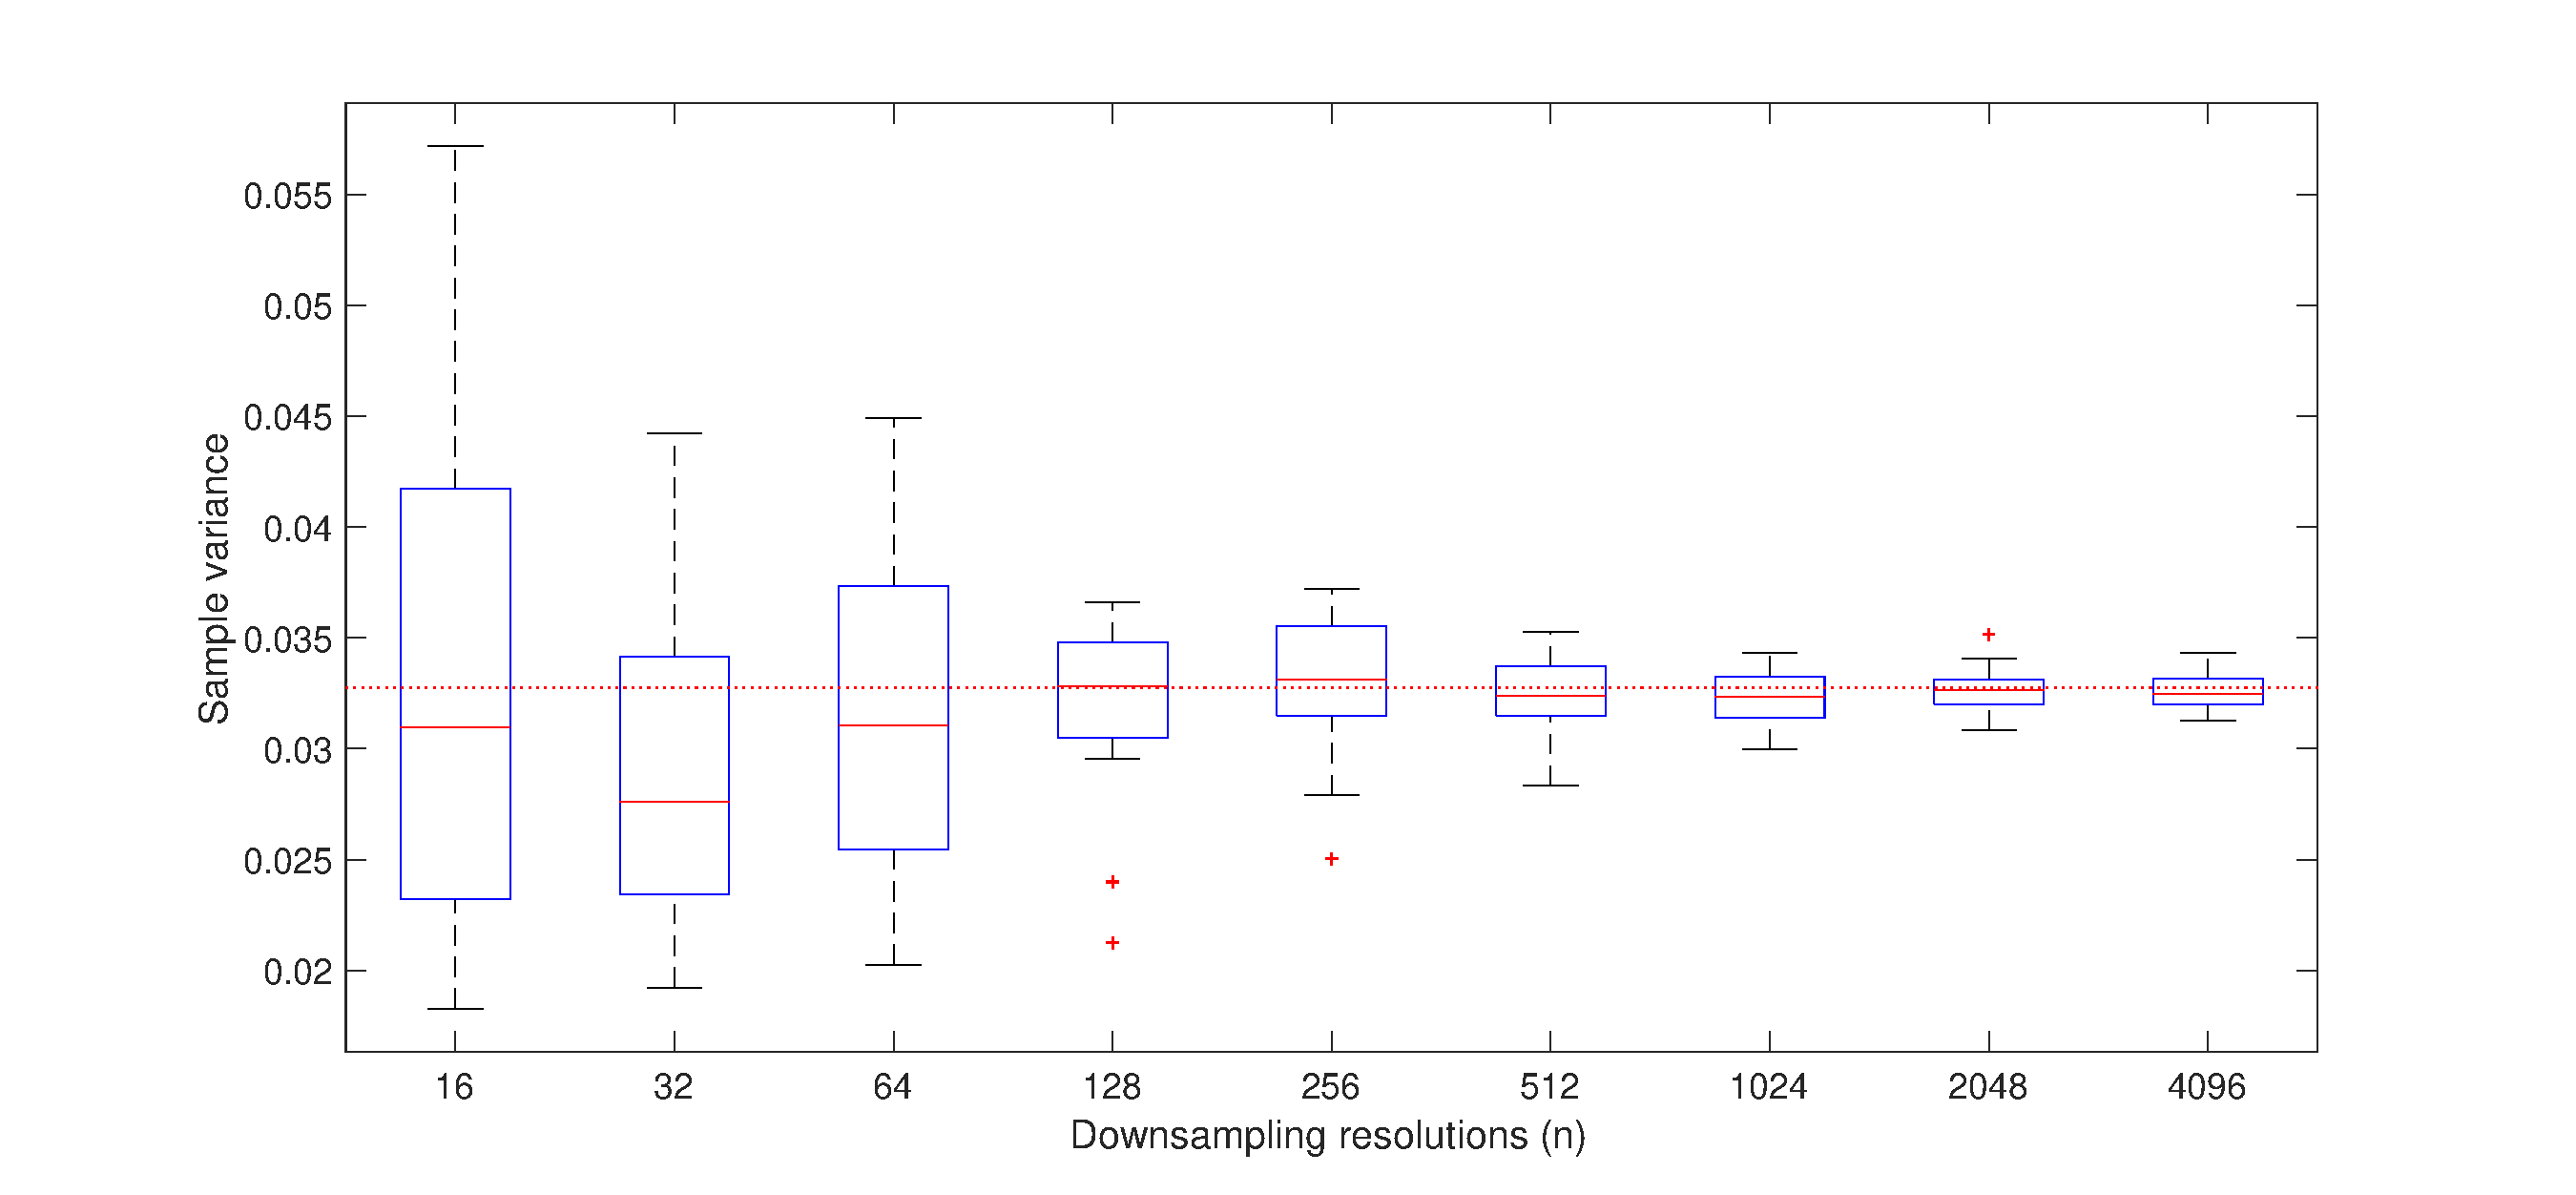
\includegraphics[scale=0.45]{Figures/VarPlot1D_F1_S05_W100_R20.eps}}
\caption{The boxplots were generated from the sample variances of downsampled noise vectors. The theoretical variance of the noise was set to 0.0327, which is indicated by the horizontal dotted line. This figure illustrates that as the lengths of the downsampled vectors decrease, the variance in the computed sample variances increases.}
\label{VarPlot1D}
\end{figure}

One description of the effects of downsampling a vector in terms of the DFT is the Downsampling Theorem \cite[Ch.~7]{AudioDFT}. Given a vector $\mathbf{x} \in \mathbb{C}^N$, where $N = LM$ for positive integers $L$ and $M$, and \textit{aliasing operator} $\alias_L(\cdot) : \mathbb{C}^N \rightarrow \mathbb{C}^M$ is defined as
\[\left(\alias_L(\mathbf{x})\right)_j = \sum_{k=0}^{L-1} x_{j+kM}, \quad \mathbf{x} \in \mathbb{C}^N, \quad j \in \{0,1,\ldots,M-1\}.\]
The vector $\alias_L(\mathbf{x})$ is is the result of partitioning the vector $\mathbf{x}$ into $L$ vectors of length $M$ and summing them. The aliasing operator is linear and thus could be defined using a matrix representation; if $L = 2$, the aliasing operator has an $M \times N$ matrix representation $A$ that has entries
\[A_{j,k} = \begin{cases}
1, & j = k \bmod M, \\
0, & \text{otherwise}
\end{cases}, \quad 0 \leq j \leq M-1, ~ 0 \leq k \leq N-1.\]
With the aliasing operator defined, the Downsampling Theorem can be stated.
\begin{theorem}{Downsampling Theorem}
Let $\mathbf{x} \in \mathbb{C}^N$, where $N = LM$ for positive integers $L$ and $M$, let $\mathbf{y} = \mathbf{x}^M$, and let $\dft{y}$ and $\dft{x}$ denote the DFT of $\mathbf{y}$ and $\mathbf{x}$, respectively. Then
\[\dft{\mathbf{y}} = \frac{1}{\sqrt{L}}\alias_L\left(\dft{\mathbf{x}}\right).\]
\end{theorem}
\begin{proof}
Since the length of $\dft{\mathbf{x}}$ is $N$, $\alias_L\left(\dft{\mathbf{x}}\right)$ has length $M = N/L$. Letting $\mathbf{z} = \alias\left(\dft{\mathbf{x}}\right)$, we have that
\[z_j = \sum_{k=0}^{L-1}\dft{x}_{j+kM}, \quad j\in\{0,1,\ldots,M-1\},\]
because each component of $\mathbf{z}$ is the sum of $L$ components of $\dft{\mathbf{x}}$. Fixing some $j\in\{0,1,\ldots,M-1\}$, the definition of the DFT and the fact that $M/N = L$ give
\begin{align*}
\sum_{k=0}^{L-1}\dft{x}_{j+kM} &= \sum_{k=0}^{L-1} \left(\frac{1}{\sqrt{N}}\sum_{\ell=0}^{N-1} x_{\ell}\exp\left(\frac{-2\pi{i}(j+kM)\ell}{N}\right)\right) \\
&= \frac{1}{\sqrt{N}} \sum_{k=0}^{L-1} \sum_{\ell=0}^{N-1} x_{\ell}\exp\left(\frac{-2\pi{ij\ell}}{N}\right)\exp\left(\frac{-2\pi{ikM\ell}}{N}\right) \\
&= \frac{1}{\sqrt{N}} \sum_{k=0}^{L-1} \sum_{\ell=0}^{N-1} x_{\ell}\exp\left(\frac{-2\pi{ij\ell}}{N}\right)\exp\left(\frac{-2\pi{ik\ell}}{L}\right) \\
&= \frac{1}{\sqrt{N}} \sum_{\ell=0}^{N-1} x_{\ell} \exp\left(\frac{-2\pi{ij\ell}}{N}\right) \left(\sum_{k=0}^{L-1} \exp\left(\frac{-2\pi{ik\ell}}{L}\right)\right).
\end{align*}
The sum over $k$ is geometric:
\[\sum_{k=0}^{L-1} \exp\left(\frac{-2\pi{ik\ell}}{L}\right) = \sum_{k=0}^{L-1} \left(\exp\left(\frac{-2\pi{i\ell}}{L}\right)\right)^k.\]
If $n = 0 \bmod L$, then the summands are all 1 and the sum is equal to $L$. If $n \neq 0 \bmod L$, then the formula for a geometric sum produces
\[\sum_{k=0}^{L-1} \left(\exp\left(\frac{-2\pi{i\ell}}{L}\right)\right)^k = \frac{1-\exp(-2\pi{i\ell})}{1-\exp(-2\pi{i\ell/L})} = 0,\]
where the last equality comes from noting that $\exp(-2\pi{i\ell}) = 1$ for all integers $\ell$. Performing the change of index $m = \ell/L$, the results regarding the sum over $k$ imply
\[\frac{1}{\sqrt{N}} \sum_{\ell=0}^{N-1} x_{\ell} \exp\left(\frac{-2\pi{ij\ell}}{N}\right) \left(\sum_{k=0}^{L-1} \exp\left(\frac{-2\pi{ik\ell}}{L}\right)\right) = \frac{L}{\sqrt{N}} \sum_{m=0}^{(N/L)-1} x_{mL} \exp\left(\frac{-2\pi{ijmL}}{N}\right)\]
because integral values of $m = \ell/L$ means that $\ell = 0 \bmod L$. Using $N = LM$ and noting that $x_{mL} = y_m$ yields
\[z_j = \frac{L}{\sqrt{N}} \sum_{m=0}^{(N/L)-1} x_{mL} \exp\left(\frac{-2\pi{ijmL}}{N}\right) = \frac{L}{\sqrt{N}} \sum_{m=0}^{M-1} y_m \exp\left(\frac{-2\pi{ijm}}{M}\right) = \frac{L\sqrt{M}}{\sqrt{N}} \dft{y}_j.\]
Therefore $\dft{\mathbf{y}} = \frac{1}{\sqrt{L}}\mathbf{z} = \frac{1}{\sqrt{L}}\alias_L\left(\dft{\mathbf{x}}\right)$.
\end{proof}
In words, the Downsampling Theorem states that the DFT of a downsampled vector is equal to a (scaled) summed partition of the DFT of the original vector. A direction of future work will be to see if the Downsampling Theorem can be directly applied to the parameter estimation functions in Chapter \ref{ch:Parameter estimation methods} to analyze the effects of downsampling on the functions themselves. \par 
Each function in Chapter \ref{ch:Parameter estimation methods} uses the assumption that noise is present in the given data. Since data in the context of the DFT are often considered discretizations of analog signals, a common quantifier of noise in data is the signal-to-noise ratio (SNR). Though the definition of SNR varies, the definition chosen for this investigation is
\begin{equation}
\label{eq:SNR}
\text{SNR} = 10\log_{10}\left(\frac{P_{\text{signal}}}{P_{\text{noise}}}\right)
\end{equation}
where $P$ denotes average power. In the discrete setting, the average power of a signal $\mathbf{f}$ of length $N$ is defined as $\|\mathbf{f}\|^2/N$. Using this definition, $P_{\text{signal}} = \|\gVec\|^2/N$ and $P_{\text{noise}} = \|\noiseVec\|^2/N$ and so the quotient in the logarithm is $\|\gVec\|^2/\|\noiseVec\|^2$. The quotient can also be expressed as $(\|\gVec\|/\|\gnoiseVec - \gVec\|)^2$, which is the square of the multiplicative inverse of the relative error of $\gnoiseVec$. \par
In MATLAB, the noise vector $\noiseVec$ can be constructed by first taking an $N$-vector $\mathbf{e}$ drawn from the multivariate standard normal distribution and multiplying the vector by a constant $\noiseSD$. Doing so ensures that $\noiseVec$ has variance $\noiseSD^2$ because $\Var(\noise) = \Var(\noiseSD\:\mathbf{e}) = \noiseSD^2\:\Var(\mathbf{e})$ and $\mathbf{e}$ has unit variance. Thus it is useful to rearrange the equation defining SNR into an equation that provides a way of finding the necessary variance for a given SNR value. The rearrangement is shown below, with $\|\noiseVec\|^2$ replaced by $\E(\|\noiseVec\|^2)$.
\[\E(\|\noiseVec\|^2) = \frac{\|\gVec\|^2}{10^{(\text{SNR}/10)}}\]
Using the properties of expected value and the fact that $\E(\|\noiseVec\|^2) = \E(\|\noiseSD\:\mathbf{e}\|^2)$, the term on the left hand side of the equation can be changed as
\[\E(\|\noiseVec\|^2) = \E(\|\noiseSD\:\mathbf{e}\|^2) = \noiseSD^2 \sum_{j=1}^N \E(\mathbf{e}_i^2) = \noiseSD^2 \sum_{j=1}^N \left(\E(\mathbf{e}_i)^2 + \Var(\mathbf{e}_i)\right) = \noiseSD^2 \sum_{j=1}^N \left(0^2 + 1\right) = \noiseSD^2\:N.\]
Utilizing this change, the following equation for variance is obtained.
\begin{equation}
\label{eq:Var}
\noiseSD^2 = \frac{\|\gVec\|^2}{N \cdot 10^{(\text{SNR}/10)}}
\end{equation}
This equation is used for the numerical construction of the noise vectors. SNR values of 5 and 25 are used to generate the white noise added to $\gVec$, and one such data realization is shown in Figure \ref{NoisePlot1D_F2_S05_W200}. \par

\begin{figure}
	\centerline{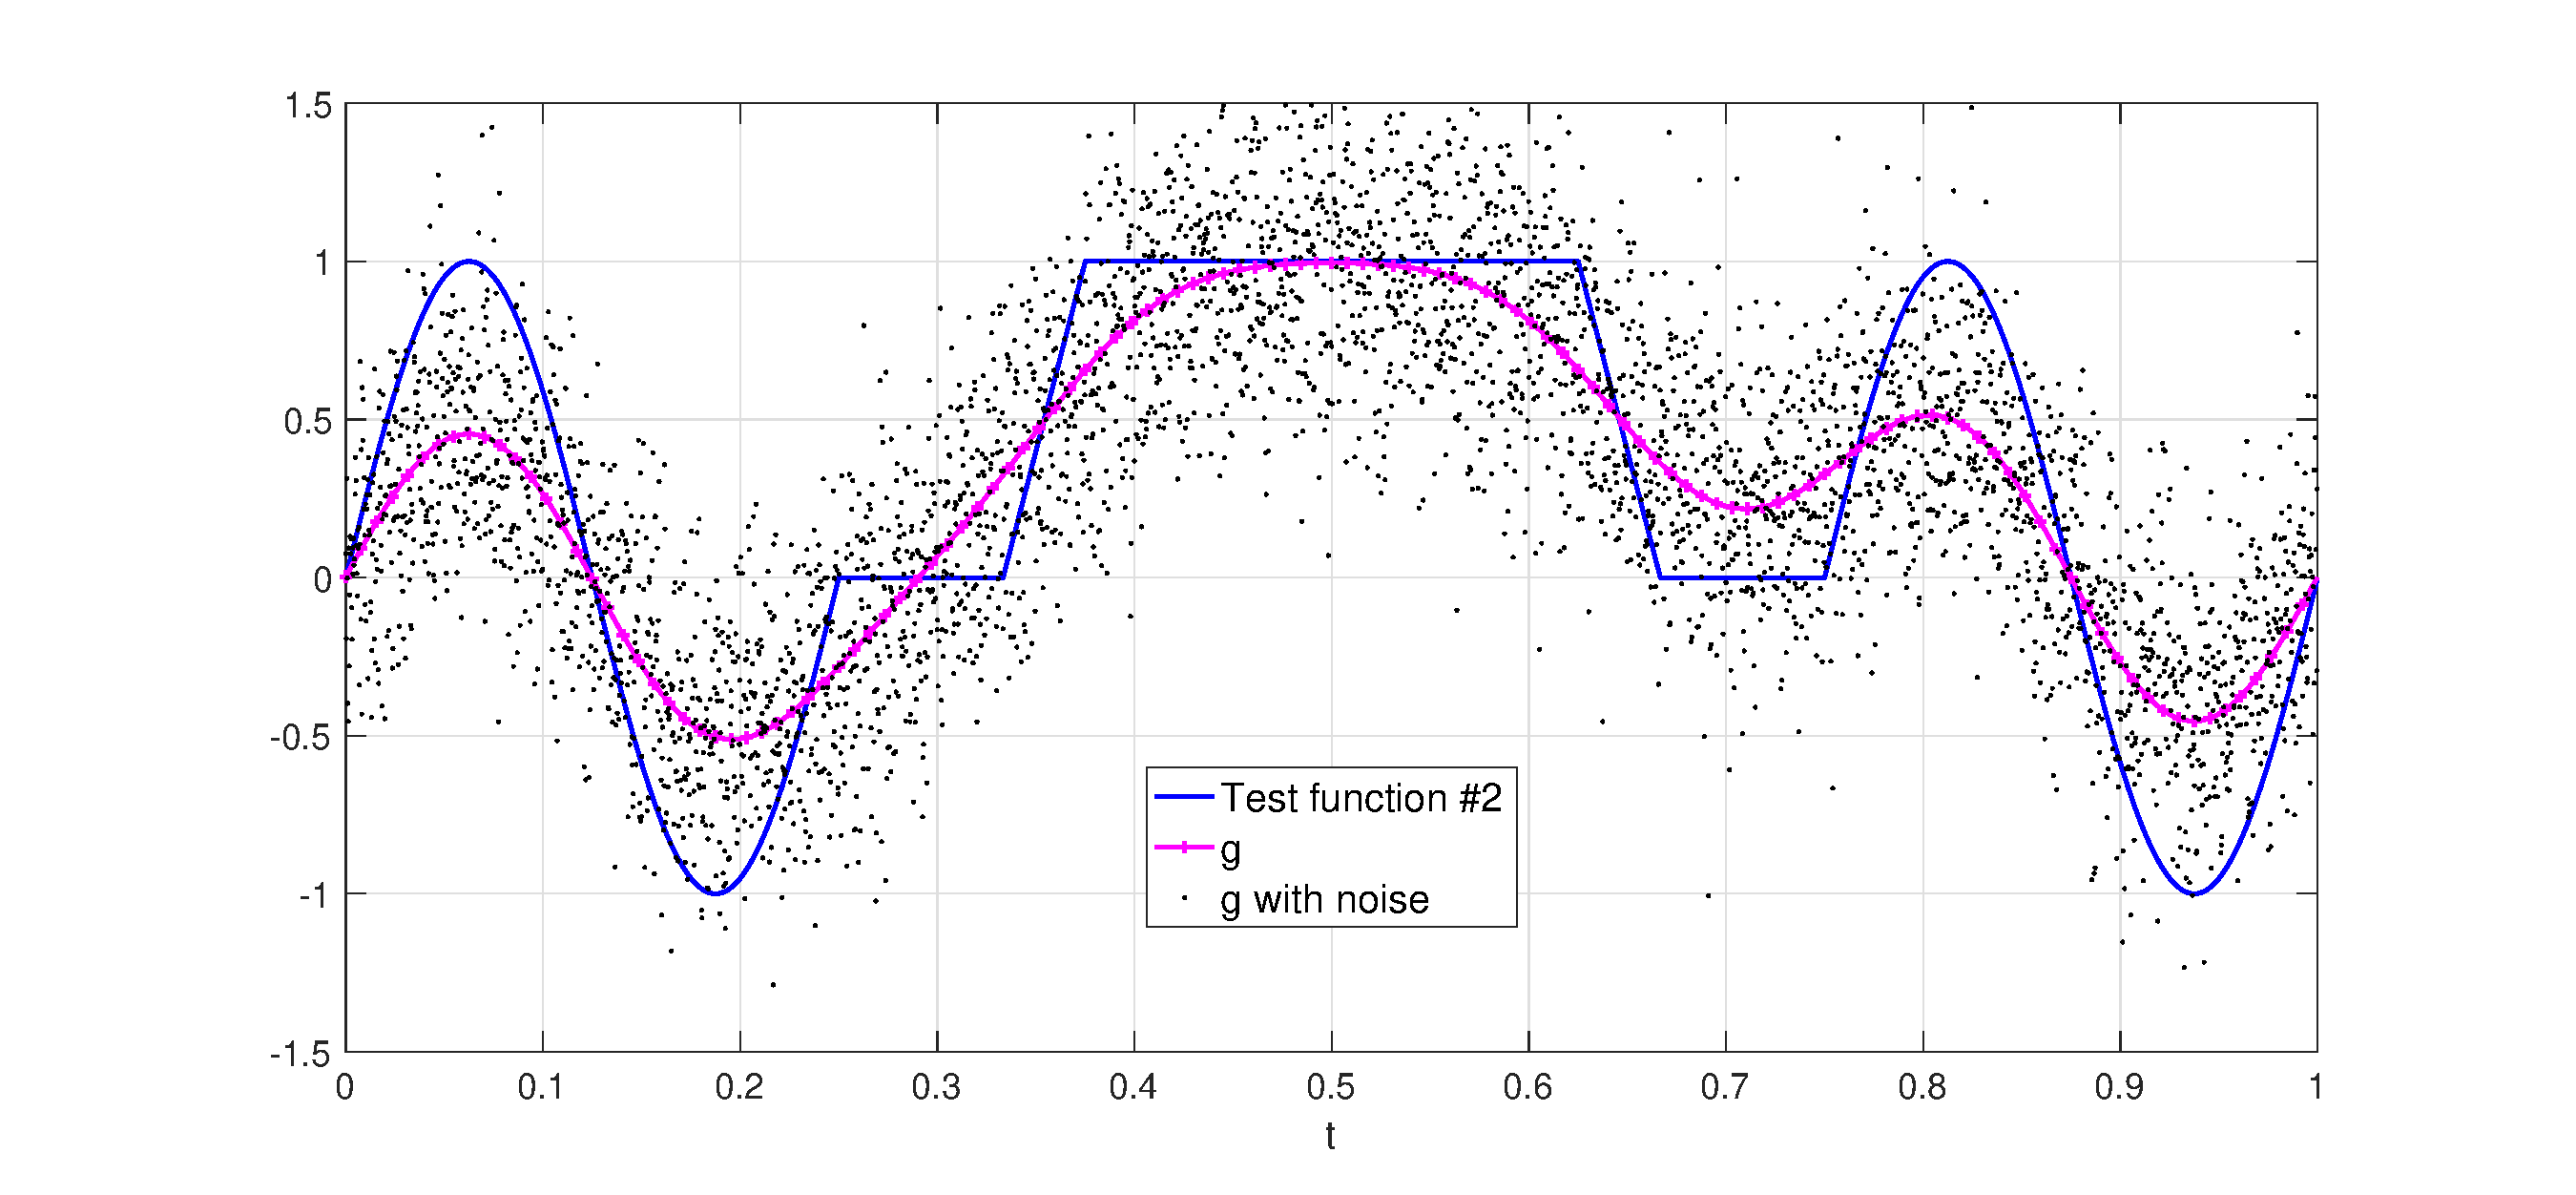
\includegraphics[scale = 0.45]{Figures/NoisePlot1D_F2_S05_W200.eps}}
\caption{The plot shows one data realization of $\gVec$ with noise, where the original function $f$ was the second test function. The SNR value is 5 and the width of the Gaussian kernel is 200.}
\label{NoisePlot1D_F2_S05_W200}
\end{figure}

For an accurate evaluation of the numerical examples and their results, multiple realizations of noise are used. A primary advantage of multiple noise realizations is that the sample variance of noise vectors approaches the desired variance as the number of realizations increases. More rigorously, the mean of the sample variances of the noise vectors converges almost surely to the expected value of the sample variance, which is the desired variance $\noiseSD^2$; this is a direct consequence of the (strong) law of large numbers and the fact that the noise vectors are independent and identically distributed with standard normal distribution.
